\documentclass[12pt, a4paper]{article}   % list options between brackets
\usepackage{blindtext}              % list packages between braces

\usepackage{fancyhdr}
\pagestyle{fancy}
%\renewcommand{\chaptermark}[1]{\markboth{\thechapter.\space#1}{}} 
%\renewcommand{\sectionmark}[1]{\markright{#1}{}}

\usepackage{listings}
\usepackage{color}
\usepackage{setspace}
\usepackage{graphicx}

% type user-defined commands here

\begin{document}

\doublespacing

\title{Project Phase 1\\Report: Design \& Screenshots}   % type title between braces
%\\ \vspace{-1.5ex}
\author{Web development Fundamentals (CMPS 350, L01) \\\vspace{-1.5ex} Mohsin Al-Ashwal 123456789, \\\vspace{-1.5ex} Mohammad Hassam Tahir Khaili 202010329, \\\vspace{-1.5ex}Syed Ahmed Subzwari 123456789, \\ Basil Saeed 202108258}         % type author(s) between braces
%\date{October 27, 1995}    % type date between braces
\maketitle
\tableofcontents
\break

\section{UI Design}             % chapter 1
Prototypes of the initial user interfaces were made using Figma.

The prototypes were made to plan the structure of the content, so the color and ``presentation" of the pages were changed, as we made better designs and colors in the actual implementation.

\begin{figure}[h]
\begin{center}
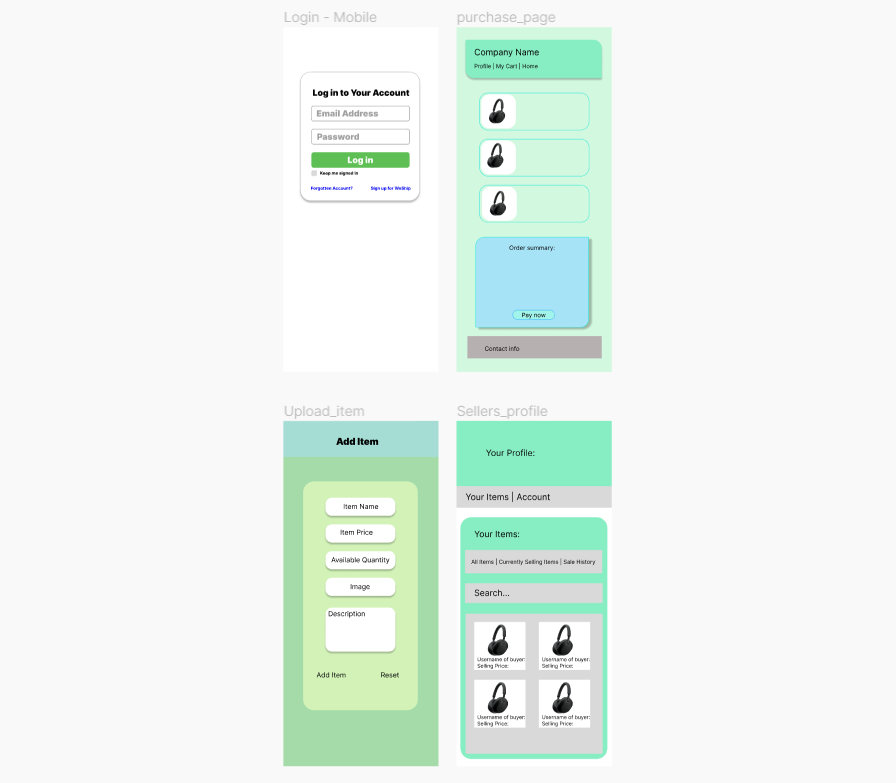
\includegraphics[width=120mm]{figmaSample.PNG}
\caption{Figma Prototype}
\end{center}
\end{figure}

\break

\section{Application Design}           % chapter 2

This section will show the UML Class Diagram for the backend of the application.

\begin{figure}[h]
\begin{center}
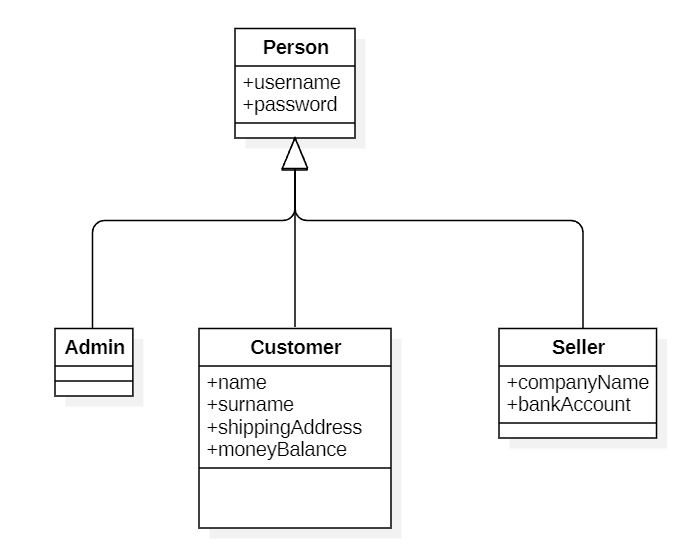
\includegraphics[width=120mm]{umlSample.PNG}
\caption{Class Diagram of the Application}
\end{center}
\end{figure}

\section{Testing (Screenshots)}

\section{Contribution Discussion}
This section contains the contribution discussion by all group members.
\subsection{\small{Mohsin Al-Ashwal}}
I made this, this and this...
\subsection{\small{Mohammad Hassam Tahir Khaili}}
I made this, this and this...
\subsection{\small{Syed Ahmed Subzwari}}
I made this, this and this...
\subsection{\small{Basil Saeed}}
I made this, this and this...
\end{document}